\documentclass{bioinfo}
\copyrightyear{2016} \pubyear{2016}

\usepackage{gensymb}
\usepackage{tikz}
\usetikzlibrary{calc}

\access{Advance Access Publication Date: 23 Oct 2016}
\appnotes{Manuscript Category}

\begin{document}
\firstpage{1}

\subtitle{Computational and Systems Biology}

\title[Model inference from protein time-course in Hematopoietic Stem Cells (HSC)]{Model inference from protein time-course in Hematopoietic Stem Cells (HSC)}
\author[Pandu Raharja, Rene Schoeffel, Michael Strasser and Carsten Marr]{Pandu Raharja\,$^{\text{\sfb 1,}\text{\sfb 2,}\text{\sfb 3,}*}$, Rene Schoeffel\,$^{\text{\sfb 1,}\text{\sfb 2,}\text{\sfb 3}}$, Michael Strasser\,$^{\text{\sfb 3}}$ and Carsten Marr\,$^{\text{\sfb 3,}*}$}
\address{$^{\text{\sf 1}}$Technische Universit\"at M\"unchen, Fakult\"at f\"ur Informatik, Boltzmannstr. 3, 85748 Garching bei M\"unchen, Germany\\
$^{\text{\sf 2}}$Ludwig-Maximilians-Universit\"at M\"unchen, Professor-Huber-Platz 2, 80539 M\"unchen, Germany\\
$^{\text{\sf 3}}$Helmholtz Zentrum M\"unchen, Institute of Computational Biology, Ingolst\"adter Landstr. 1
85764 Neuherberg, Germany.}

\corresp{$^\ast$To whom correspondence should be addressed.}

\history{Received on 23/09/2016; revised on 14/10/2016; accepted on 21/10/2016}

\editor{Associate Editor: Jan Quell}

\abstract{\textbf{Motivation:} 
Unlike averaged effect commonly found in aggregate cells population data, the dynamics of single cell strongly exhibits the stochasticity of gene expression. These stochastically influenced dynamics in gene expression appears to convey more information about the background mechanism of gene expression routines than it would be otherwise understood through the study of population average.\\
\textbf{Results:}In this paper we presented a particle filtering-based algorithm and a framework that is capable of inferring parameters underlying the stochastic models from single cell expression data. This framework was then applied on time-lapsed microscopy data of two transcription factors (\texttt{Pu.1} and \texttt{Gata.1}) in murine blood stem cells. It is thought that both transcription factors play decisive roles in several stages of stem cell differentiation, especially the differentiation of hematopoetic stem cells. Our results provide several insights into the dynamics of blood stem cells maturation and specifically in the single cell environment. We managed to gain several valuable insights on the interaction dynamics between two transcription factors and the outcome of cell maturation. While doing so, we managed to developed highly flexible general purpose highly parallelized framework to model dynamical systems using particle filtering. The general framework software is now available as free software for anyone to use.\\
\textbf{Availability:} The data are available upon request. A general framework for determining the parameters that best explain the data were published under open source license. The complete source code of the program is publicly accessible at \href{https://github.com/raharjaliu/PFInfer}{https://github.com/raharjaliu/PFInfer}.\\
\textbf{Contact:} \href{pandu.raharja@tum.de}{pandu.raharja@tum.de}\\
\textbf{Supplementary information:} Supplementary data are available at \textit{Bioinformatics}
online.}

\maketitle

\section{Introduction}

The advances in gene expression measurement techniques, coupled with equally rapid advances in single cell analytics, have allowed the more recent high resolution single cell analysis of cell dynamics \citep{Feigelman16, Hoppe16}. This has enabled us, for example, to look deeper into the dynamics of stem cell maturation. In recent years alone, several genes that potentially are involved in the decision making mechanism of cell maturation going from Inner Mass Cell (IMC) all the way to somatic cells have been discovered and widely known by now \citep{Graf09}. While this has enable us to study cell processes more thoroughly, the deterministic population-averaged nature of cell dynamics was becoming less and less apparent while the stochastic nature of single cell dynamics was becoming dominating as the analysis went down onto single cell resolution \citep{Elowitz02}. Hence our motivation to apply inference methods that are capable to infer dynamics of the systems that are heavily influenced by non-deterministic factors.

For this project we use particle filtering to learn more about aforementioned dynamics. We apply this technique on our time-dependent expression data of single cells containing concentration of both transcription factors. The approach of the experiment would be further described in the next section followed by the theoretical aspects of the particle filtering and other methods used in this project.

In this paper we focus on the maturation lines of hematopoietic stem cells \citep{Orkin08}. The lines start with Long Term Hematopoietic Stem Cells (LT-HSC), which is progenitor of all blood cells. During its life, LT-HSC could either divide into two LT-HSC or turn into Short Term Hematopoietic Stem Cell (ST-HSC). SH-HSC will then undergo a transition process into either Common Myeloid Progenitor (CMP) or Common Lymphoid Progenitor (CLP). As the names suggest, both cells are the ancestor of all myeloid cells and lymphocites, respectively. Each would then further maturate into their respective intermediate cells and eventually the mature somatic cells (Red Blood Cells, Megakaryocytes, Mast Cells, Eosinophils, Neutrophils and Macrophages from CMP and B and T Lymphocytes from CLP; see Figure \ref{fig:01}).

The decision process of CMP transitioning into either MEP and GMP stands in focus of our project. Two transcription factors, \texttt{Pu.1}and \texttt{Gata.1} are thought to influence the decision process \citep{Graf09}. Moreover, both transcription factors are known to inhibit each other. It is thought that the whole cross inhibition dynamics between the two has an impact on the fate of Common Myeloid Progenitor. This dual-agent dynamics is thought to behave in a way that is self-fulfilling. That is, a slight change in concentration of transcription factors favoring one state over another will have stupendous impact on cell fate decision \citep{Filipczyk15}.

\begin{figure}[h]
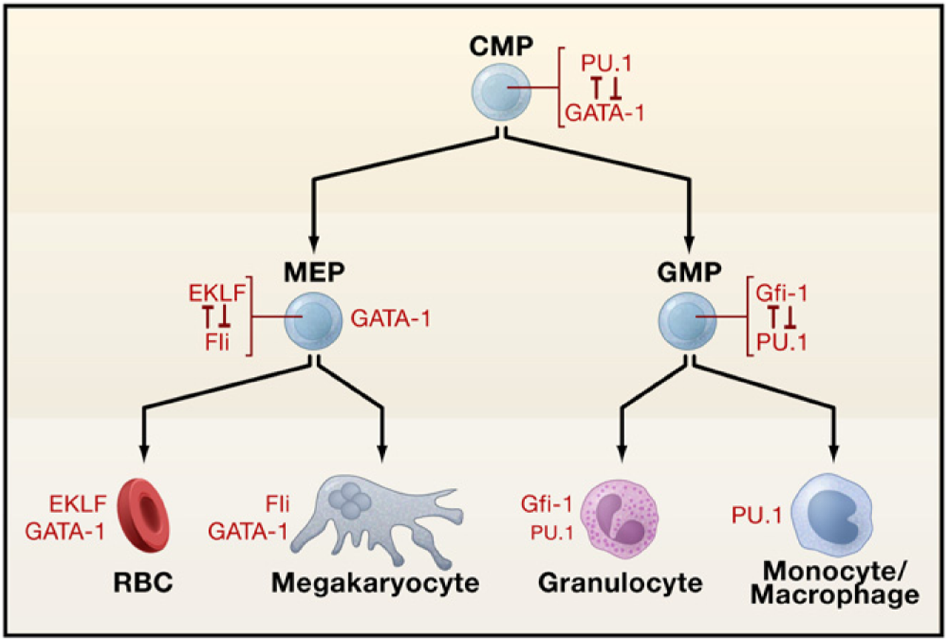
\includegraphics[width=8cm]{figures/homatopoietic_focus}
\caption{Maturation cascade of intermediate Common Myeloid Progenitor (CMP) to Megakaryocyte-Eerythroid Progenitor (MEP) and Granulocyte/Macrophage Progenitor (GMP). MEP would then maturate into somatic Red Blood Cells and Megakaryocites while GMP would undergo maturation into Granulocytes and Monocyptes. For each process there are known factors which are known to interact antagonistically on maturation decision. Our CMP to MEP and GMP decision stands on the top of the figure with two transcription factors of interest, \texttt{Pu.1} and \texttt{Gata.1} interact atagonistically. Figure taken from \citealp{Graf09}.}\label{fig:01}
\end{figure}

\section{Approach}

For the single cell dynamic analysis to be possible, we were interested in gaining insight in single cell transcription data of both \texttt{Pu.1} and \texttt{Gata.1}. We combine two techniques for this to be possible: single cell tracking and protein tagging.

\subsection{Experimental Setting}

The data for the experiment were taken from Hoppe {\it et~al}, 2016 \citep{Hoppe16}. The expressed protein of interests \texttt{Pu.1} and \texttt{Gata.1} were tagged with distinct fluorescence proteins \texttt{eYFP} and \texttt{mCherry} respectively. Time-wise expression levels were then measured based on the intensity of aforementioned florescence proteins.

Time-lapse imaging was performed at 37 $^{\circ}$C in fibronectin coated channel slides provided by Takara Bio. The light source for the experiment was a HXP 120 from Zeiss. 46HE and 43HE, both provided by Zeiss, were used to detect eYFP and mCherry fluorescence coming from the cells at exposure times between 400-1,500 ms using an AxioCam HRm from Zeiss. Bright field pictures were taken every 60-120 s while fluorescent pictures used for the measuring \texttt{PU.1-eYFP} and \texttt{GATA1-mCherry} were acquired every 30 min. Pictures used for analysis were saved in lossless TIF or PNG format. Single-cell tracking and image quantification were performed using self-written software as described

Figure \ref{fig:02} shows how the dataset from similarly conducted experiment taken from Feigelman, 2016 \citep{Feigelman16} visually look like.

\begin{figure}[h]
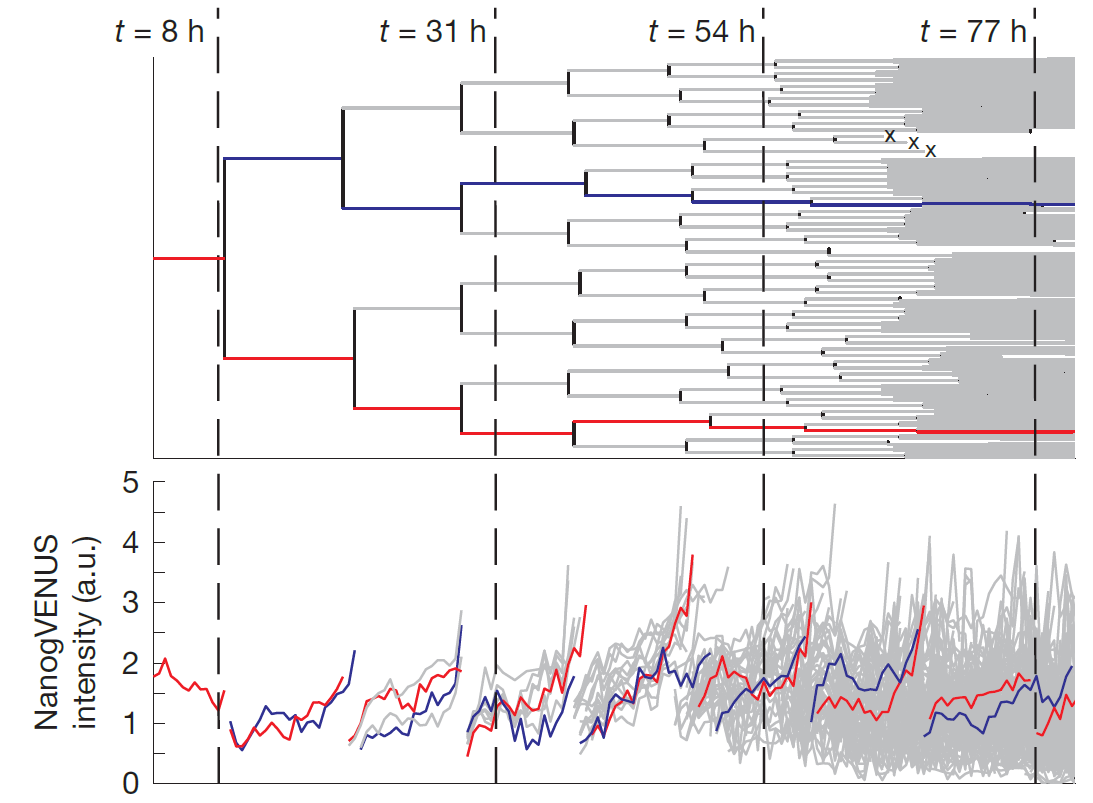
\includegraphics[width=8cm]{figures/cell-generations.png}
\caption{Example of single cell expression data. In this example, initially only one cell is observed under the bright-field and ultraviolet recording. The cell would then divide into two other cells. The system automatically recognizes this and separate measurements of expression would then be conducted, which is visible in the lower part of the figure. The above example also makes point of the uniqueness and tracability of each cell by pointing two specific lineages within the data: the blue and red lineages. The system records complete expression measurement of the lineages which could be seen in second half of the figure corresponding with the first half of the figure. The system is capable of recording not only cell division but also cell deaths, as can be seen through the x's sign in the upper part of the figure. Figure taken from \citealp{Feigelman16}.}\label{fig:02}
\end{figure}

\section{Models}

We utilize particle filtering to learn the dynamics of maturation of Common Myeloid Progentior (CMP) cells. The definition of particle filtering could be seen in the subsection \textbf{Particle Filtering}. \textbf{Simulation Process} details how the simulation would be done and the probabilistic approaches used in it. The assumed model of the cell maturation is then described in the subsection \textbf{Reaction Models}. For comparison purpose, a framework for model comparison is also presented in subsection \textbf{Models Comparison}. This is especially helpful for comparing the default model described in \textbf{Reaction Models} and other possible alternative models.

\subsection{Particle Filtering}

Particle filtering, which in several more recent literature is also known as \textbf{Sequential Monte Carlo} (SMC) \citep{Doucet01, Liu98}), is a class of methods generally used to solve the filtering problem. Classically, filtering problem is the problem of identifying best estimate of some system given noisy and incomplete input -- hence the word filter \citep{DelMoral96}. As the alternative name implies, it is a set of methods that run Monte Carlo sequentially interrupted by inference phase. It consists mainly of two phase steps, \textbf{prediction-updating} and \textbf{mutation-selection}, that are done sequentially and repetitively. In the first phase, the prediction-updating done updates the conditional probability of underlying assumption -- generally referred to as \textbf{posterior distribution} -- of a system given the previous simulation. Later on, a simulation (mutation) is done on given underlying assumption and simulations best fit the data would then be selected to update the underlying assumption in the next prediction-updating step \citep{DelMoral12}.

As the name also implies, particle filtering utilizes the use of particle, an abstract representation of combination of model, data and parameters. In the next part we will dive deep into the theory of particle filtering. First, we will define what a particle is. This is then followed by definition of Propensity, Posterior, Parameters and Prior. Finally the section will be closed by short review of other methods that also tried to stochastically infer parameters on time-lapsed fluorescent single cell data.

\subsubsection{Particle}

A particle $\mathcal{K}$ is defined as a triple of trajectory $X$, parameter set $\theta$ and assumed model $\mathcal{M}$,

\begin{equation}
\mathcal{K} := (X, \theta, \mathcal{M})\label{eq:01}
\end{equation}

Specifically in our case, trajectory refers to the concentration of measured proteins \texttt{Pu.1} and \texttt{GATA1} while parameter set encompasses all variables that were involved in the reaction such as propensity and its corresponding auxiliary variables (see subsection \textbf{Reaction Models}). Note that a trajectory is different from the experimental data $\mathcal{D}$. A trajectory is the result of the simulation done by applying the parameters onto our model. In functional notation we would assume the i-th value of the trajectory $X_i$ to be a function of the i-th value of the trajectory, the model and the parameters,

\begin{equation}
X_i = f(X_{i - 1}, \mathcal{M}, \theta_{i - 1})\label{eq:02}
\end{equation}

\subsubsection{Propensity}

As the name suggests, propensity is measure of a certain thing would be happening in a given time. In our model specifically, a propensity roughly corresponds to the chance of a reaction to happen in a given time,

\begin{equation}
a_i \propto P(R_k = r_i)
\end{equation}

Where $P(R_k = r_i)$ refers to the probability of reaction at time point k to be the -th reaction. For reactions $r_1, r_2, \cdots r_p$ there are propensities $a_1, a_2, \cdots a_p$ that are uniquely assigned to each reaction. The probability of a reaction $r_i$ to happen in a given time is thus the ratio between its propensity $a_i$ to the total sum of all propensities,

\begin{equation}
P(R_k = r_i) = \frac{a_i}{\sum_{j=0}^{p} a_i}
\end{equation}

In our model, two kinds of propensities were defined. For uninhibited reaction, i.e. a reaction in which no inhibiting effect from other species -- a term denoting any entity that is involved in a reaction network -- is assumed, the reaction specific propensity is defined as the parameter in the mass action law of chemical reaction:

\begin{equation}
a_i = k_i \label{eq:23}
\end{equation}

with $k_i$ referring to the reaction parameter of $r_i$.

For reaction $r_i$ inhibited by a species $Y$, Michaelis-Menten inhibition kinetics is assumed to be the propensity of the reaction,

\begin{equation}
a_i = k_i \cdot (1 - \frac{X_i^{n}}{X_i^{n} + K_{Y}^{n}})\label{eq:24}
\end{equation}

where $k_i$, $X_i$ and $K_{Y}$ refer to reaction parameter of $r_i$, concentration of product $X$ in a given time and inhibiting coefficient of regulator $Y$ on $X$ respectively.

\subsubsection{Posterior}

Our posterior describes the probability of having the trajectory $X$ and parameter $\theta$ given the observation $\mathcal{D}$,

\begin{equation}
P(X, \theta | \mathcal{D})\label{eq:03}
\end{equation}

This is understood as the probability of having our simulation return a given set of values \textit{and} having the parameter set $\theta$ given that we previously observed the experimental data $\mathcal{D}$. Using Bayes' Theorem we could further expand our posterior into an update rule,

\begin{equation}
P(X, \theta | \mathcal{D}) = \frac{P(\mathcal{D} | X, \theta)  P(X, \theta)}{P(\mathcal{D})}\label{eq:04}
\end{equation}

In the simulation it is well known that, to compute prior $P(\mathcal{D} | X, \theta)$, only knowledge about the trajectory of the simulation is needed \citep{Feigelman16}. Hence, the prior could be simplified as,

\begin{equation}
P(\mathcal{D} | X, \theta) = P(\mathcal{D} | X)\label{eq:05}
\end{equation}

Note that the above equation inherently assumes that $\mathcal{D}$ is only directly dependent on $X$ and $X$ is in turn only directly dependent on $\theta$. Incorporating this onto our update rule, and expanding the definition of $P(X, \theta)$ using chain rule, we get

\begin{equation}
P(X, \theta | \mathcal{D}) = \frac{P(\mathcal{D} | X)  P(X | \theta) \pi(\theta)}{P(\mathcal{D})}\label{eq:06}
\end{equation}

One of the interesting aspects of our method is the fact that the i-th simulation result is only dependent on previous simulation, a property known as \textit{Markov property}. We could thus rewrite the update rule as follow,

% TODO correct the second product definition. It seems off

%\begin{equation}
%P(X, \theta | \mathcal{D}) = \frac{\prod_{i=0}^{N} P(\mathcal{D}_i | X_i) P(X_0) \prod_{l=1}^{N} P(X_{[t-1, ti]} | X_i, \theta)\pi(\theta)}{P(\mathcal{D})}\label{eq:07}
%\end{equation}

\begin{equation}
P(X, \theta | \mathcal{D}) = \frac{\prod_{i=0}^{N} P(\mathcal{D}_i | X_i) P(X_0) \prod_{l=1}^{N} P(X_{[tl-1, tl]} | X_l, \theta)\pi(\theta)}{P(\mathcal{D})}\label{eq:07}
\end{equation}

\subsubsection{Parameters}

During the simulation we assumes certain parameters that would influence the trajectory of the simulation. The parameter set $\theta$ could then mathematically be understood as P-tuple containing all the parameters that are assumed in the simulation,

\begin{equation}
P := (P_0, P_1, \dots , P_P)\label{eq:08}
\end{equation}

\subsubsection{Prior}

Our prior $\pi(\theta)$ could be expanded by assuming the independence of each parameter $\theta_i$ within the parameter set $\theta$,

\begin{equation}
\pi(\theta) = \prod_{i=1}^{P} \pi(\theta_i)\label{eq:09}
\end{equation}

Specifically for this simulation, we assume our prior to be gamma distributed with the parameters $\alpha$ and $\beta$,

\begin{equation}
\pi(\theta) = \prod_{i=1}^{P} Ga(\theta_i, \alpha_i, \beta_i)\label{eq:10}
\end{equation}

We used gamma distribution as our prior due to the fact that a conjugate prior of a gamma distributed random variable is also gamma distributed.

\subsubsection{Comparison with other methods}

There are several methods that infer stochastic processes. Wilkinson -- and later on, Golightly and Wilkinson --  inferred stochastic differential equation (SDE) kinetic model of bacterial gene regulation using likelihood-free Markov Chain Monte Carlo (MCMC) on florescence data \citep{Wilkinson10, GolightlyWilkinson10}. Gonzales \textit{et al} did two stochastic inference methods, Mixed Effects (ME) and the Chemical Master Equation (CME), on time-lapsed single-cell data. The paper also tested the method by inferring previously known HOG pathway in yeast \textit{Saccharomyces cerevisiae} \citep{Gonzales13}. Koromowski \textit{et al} developed Bayesian framework performed using Markov Chain Monte Carlo (MCMC) and linear noise approximation to calibrate models on fluorescent experiment data \citep{Komorowski09}.


\subsection{Simulation Process}

The simulation is run in roughly following high level steps:

\begin{enumerate}
\item Initialization of parameters $\theta$.
\item Input of data $\mathcal{D}$.
\item Particle filtering routine:

\begin{enumerate}
\item Generation of initial particles for step i

\begin{equation}
Ki := (K_{i1}, K_{i2}, \dots, K_{im})\label{eq:11}
\end{equation}

\item Simulation run of each particle $K_{ij}$
\item Weighting of each particle. The weight is a function of probability of observing the data given the simulation result.

\begin{equation}
w_i^k = P(D_i | X_i^k) = \mathcal{N}(\mathcal{D}_i | X_i^k)\label{eq:12}
\end{equation}

\item Parameter update for every K,

\begin{equation}
\theta^k \propto P(\theta | X^k_{[to, ti]})\label{eq:13}
\end{equation}

\end{enumerate}

\item Model comparison. This could be done by utilizing measures such as Akaike Information Criterion, Bayesian Information Criterion and Bayes Factor \citep{PosadaBuckley14, Bozdogan87}.

\end{enumerate}

The visualization of the whole particle filtering process could be seen in Figure \ref{fig:03}.

\begin{figure}[h]
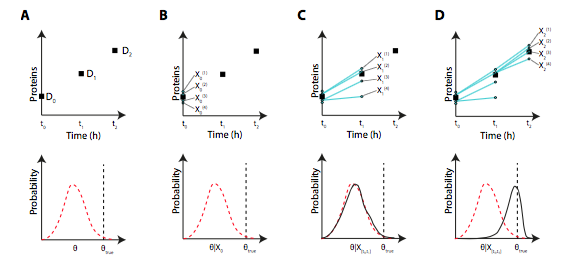
\includegraphics[width=8cm]{figures/particle_filtering.png}
\caption{Visualization of particle filtering. (A): The particle filter requires a series of observation $\mathcal{D} = (\mathcal{D}_0, \mathcal{D}_1, \cdots \mathcal{D}_N)$ (top) and a prior distribution for model parameters $\pi(\theta)$ (bottom) as input. (B): Particles are initialized by sampling initial states $X(K)$ for each particle $K$. Parameters $\Theta$ are sampled from the prior distribution $\pi(\theta)$. (C): The trajectories are resampled according to the likelihood $w_0^{(k)} = P(D_0|X_0(k))$ and propagated to the next time step using stochastic simulations to generate new states $X_1^{(k)}$ at timepoint $t_1$. Model parameters for each latent trajectory are resampled from the conditional distribution $P(\theta|X^{(k)}_{[t0,t1]})$. (D): At each iteration, the weights are recomputed and the particles are resampled. Resampled particles are propagated to the next timepoint and the parameters are resampled conditional on the resampled latent trajectories. Over time the posterior parameter distribution converges to the true value. Figure taken from Feigelman, 2016 \citealp{Feigelman16}}  \label{fig:03}
\end{figure}

\vspace*{-6pt}

\subsubsection{Particle Generation}

As mentioned before, A particle $\mathcal{K}$ is defined as a 3-tuple of trajectory $X$, parameter set $\theta$ and assumed model $\mathcal{M}$. For a specific model, j-th particle at i-th time particle is then just a tuple of trajectory and parameter set $k_{ij} = (x_i, \theta_{ij})$.

For initial time, a particle could be constructed by combining initial parameters, which were arbitrarily defined by a pre-defined prior, and initial trajectory value $X_0$. There are three ways to define the initial trajectory value. First is to take 0 as initial value. Second is to take the first measurement data $\mathcal{D}_0$. Third is to model initial data as normal distributed instances around $\mathcal{D}_0$, i.e. $X_0 \propto \mathcal{N}(\mathcal{D}_0)$. It is worth noting that the first strategy may not always be applicable.

M particles would then be created and for each iteration of the simulation with each particle having weight which calculated from previous iteration $w_{i - 1}^k$. In the next iteration, M particles are to be chosen. Note that this implies that a particle from previous iteration could be chosen more than once. Corollarly, a particle from previous iteration may also not be chosen at all. The draw is done by first drawing a random $z \propto \mathcal{U}(0, 1)$. A particle $k_{ij}$ is chosen with j denoting the smallest index so that the sum of all weight of particles with index smaller than j is larger than z, i.e.

\begin{equation}
\sum_{l=1}^{j} w_{i - 1}^l \geq z\label{eq:14}
\end{equation}

\subsubsection{Simulation Run}

Simulation is done using Gillespie's SSA algorithm, named after Daniel Thomas Gillespie (\citealp{Gillespie77}). Dating back to as early as 1945, when it was developed by Joseph Doob \citealp{Doob45} \citealp{Chung67}, moden Gillespie implementation includes improvements developed years after the invention of the algorithm such as $\tau$-leaping and Bayesian Approximation Method. Such improvements are generally essential since it would reduce computational cost of the simulation and in turn enable the simulation to scale further to accommodate more leveraged simulation -- in our case we could simulate more cells at the same time in possible more fine-grained time-resolved manner. In our case especially, such improvements are needed to accommodate the explosion of the number of cells within our culture. Specificallt, an approximative method would prevent a bottleneck in simulation caused by the exponential increase of the number of living cells that have to be simulated.\\

\textbf{Tau Leaping}

Generally, tau-leaping works by performing all reactions happening for an interval of length tau before updating the parameters and propensity function. By allowing this kind of approximation we potentially allow more efficient simulation and thus increase the capability of the simulation to cope with larger systems. In our case, we use following tau,

\begin{equation}
\tau = \frac{1}{a_0} ln \Gamma\label{eq:15}
\end{equation}

with $a_0$ referring to total sum of reaction propensities and $\Gamma$ being uniformly distributed between 0 and 1. 

\subsubsection{Particle Weighting}

Upon the completion of all simulations within one iteration, the quality of each simulation (and in turn, the particle) will be quantified. This quantification is implied in the weighting of the particle at the next iteration $w_{i}^k$. We assume the Gaussian distribution of particle around the measurement time at time $t=i$. Using this assumption, we can quantify our weight in following manner,

\begin{equation}
w_i^k = P(\mathcal{D}_i | X_i^k) = \mathcal{N}(\mathcal{D}_i | X_i^k)\label{eq:16}
\end{equation}

%To generate particle for next iteration we utilize, however, the normalized particle weight,

%$$w_j^k = \frac{w_j^k}{\sum_{l=1}^{M} w_{j}^l}$$

\subsubsection{Parameters Update and Gamma Distribution}

After each run, the parameters would then be updated using the underlying Gamma Distribution. For $k$-th particle, the updated parameters at time $i$ are dependent on previous parameters given the trajectory of data in $[t_0, t_i]$,\\

\begin{equation}
\Theta^k \propto P(\Theta | X_{[t_0, t_i]})\label{eq:17}
\end{equation}

Applying Bayes' Rule on the probability and independent assumption, we get following equation,

\begin{equation}
P(\Theta | X) = \frac{P(X | \Theta)}{P (X)} \prod_{i} P(\Theta_i)\label{eq:18}
\end{equation}

The Gamma Distribution is particularly favored for the update since a conjugate prior of Gamma Distribution is in turn Gamma distributed,

\begin{equation}
P(\Theta | X) = \frac{P(X | \Theta)}{P (X)} \prod_{d=1}^{P} Ga(\Theta_d, \alpha_d, \beta_d)\label{eq:19}
\end{equation}

With $\alpha$ and $\beta$ referring to both the shape and rate of the distribution respectively. Owing to the fact that conjugate prior of Gamma Distribution is also Gamma distributed, this could be then further simplified as an update rule of the Gamma distribution,

\begin{equation}
P(\Theta | X) = \frac{P(X | \Theta)}{P (X)} \prod_{d=1}^{P} Ga(\Theta_d, \alpha_d + r_d, \beta_d + Gd)\label{eq:20}
\end{equation}

$r_d$ here refers to the number of times the d-th reaction was fired during the run and $G_d$ is defined as follows,

\begin{equation}
G_d := \frac{1}{k_d} \sum_{l=0}^{i} a_{l}(X(S))\label{eq:21}
\end{equation}

Here, $k_d$ and $a_{l}(X(S))$ refer to reaction rate of the d-th reaction and trajectory-dependent propensity function, respectively.

\subsection{Reaction Models}

We assume following putative cross inhibition between genes \texttt{Pu.1} and \texttt{Gata.1} playing roles in cell differentiation dynamics:

\begin{center}
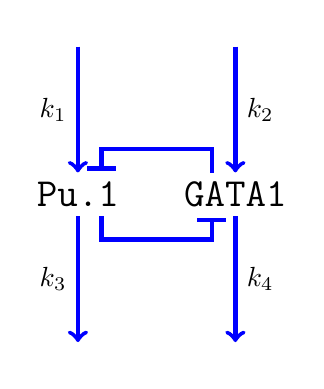
\begin{tikzpicture}[node distance=2cm]

\node (N0) {\Large $\varnothing$};
\node [right of = N0] (N1) {\Large $\varnothing$};
\node [below of = N0] (R0) {\Large \texttt{Pu.1}};
\node [below of = N1] (R1) {\Large \texttt{GATA1}};
\node [below of = R0] (N2) {\Large $\varnothing$};
\node [below of = R1] (N3) {\Large $\varnothing$};

\draw [->,ultra thick,blue] (N0) -- node[left, black] {$k_1$} (R0);
\draw [->,ultra thick,blue] (N1) -- node[right, black] {$k_2$} (R1);
\draw [->,ultra thick,blue] (R0) -- node[left, black] {$k_3$} (N2);
\draw [->,ultra thick,blue] (R1) -- node[right, black] {$k_4$} (N3);

\draw [-|,ultra thick,blue]
($ (R0) + (3mm,-2.75mm) $)
-- +(0,-3mm) %node[below, black] {$v_3$}
-| ($ (R1) - (3mm,3mm) $) ;

\draw [-|,ultra thick,blue]
($ (R1) + (-3mm,2.75mm) $)
-- +(0,3mm) %node[above, black] {$v_3$}
-| ($ (R0) - (-3mm,-3mm) $);

\end{tikzpicture}
\end{center}

There are four possible reactions happening within our model: $k_1$, $k_2$, $k_3$ and $k_4$. In our simulation, each reaction was assigned propensity value which roughly is proportional to the likelihood of the reaction happening in a given time:

\begin{equation}
P(R_i = k_l) \propto a_l\label{eq:22}
\end{equation}

The propensity $a$ of decay reactions $k_3$ and $k_4$ roughly follows the mass action law of chemical reaction:

\begin{equation}
a_l = k_l \cdot A {;} \; l \in [3, 4]\label{eq:23}
\end{equation}

For production reactions $k_1$ and $k_2$ we assume Michaelis-Menten inhibition kinetics that influences the production of the species. In this assumption, the inhibiting characteristics of a species on another species negatively influences the creation rate of the species it inhibits. The propensity of the reactions are thus,

\begin{equation}
a_1 = k_1 \cdot (1 - \frac{\texttt{GATA1}^{n}}{\texttt{GATA1}^{n} + K_{P1}^{n}})\label{eq:24}
\end{equation}

\begin{equation}
a_2 = k_2 \cdot (1 - \frac{\texttt{Pu.1}^{n}}{\texttt{Pu.1}^{n} + K_{P2}^{n}})\label{eq:25}
\end{equation}

With $K_{P1}$ and $K_{P2}$ referring to the respective protein concentrations at which inhibiton trough \texttt{GATA1} or \texttt{Pu.1} is at half its maximum effect.

\subsection{Models Comparison}

Our framework enables us to test not only standard hematopoietic stem cell maturation as described above, it also allows us to compare it with other models. One method that could be used to compare models is Bayes Factors. It is done by performing ratio of the posterior probabilities of two models $M_1$ and $M_2$,

\begin{equation}
B_{M1, M2} = \frac{P(M_1 | \mathcal{D})}{P(M_2 | \mathcal{D})}\label{eq:26}
\end{equation}

Using Bayes' Theorem, we can formulate the marginal probability as,

\begin{equation}
P(M | \mathcal{D}) = \frac{P(\mathcal{D} | M) P(M)}{P(\mathcal{D})}\label{eq:27}
\end{equation}

The marginal likelihood of model $P(\mathcal{D} | M)$ could be approximated using the particles at each iteration i (\citealp{Wilkinson11}). Since the observation of particles only depends on the previous particle, We could therefore rewrite the term as,

\begin{equation}
P(\mathcal{D} | M) = P(\mathcal{D_0}) \prod_{l=1}^{N} P(\mathcal{D}_{i+1} | \mathcal{D}_{0:i}, M)\label{eq:28}
\end{equation}

Assuming a priori equally likely models, the factor of $P(M)$ in (\ref{eq:26}) cancels between the two models and the Bayes Factors now becomes the ratio of two marginal likelihood,

\begin{equation}
B_{M1, M2} = \frac{P(\mathcal{D} | M_1)}{P(\mathcal{D} | M_2)}\label{eq:29}
\end{equation}

\section{Result}

The particle filter algorithm was applied to a time series data set containing the cell lineage of a murine stem cell. Each edge in the time series tree was simulated using 50 Particles. For each of the 41 stem cells present at the end of the experiment 50 Particles were sample according to their weights. The parameters from each chosen Particle were combined resulting in gamma distribution for each of the 6 Parameters. These gamma distributions represent the described posterior (Equation \ref{eq:03}) and their expected value is the optimal fit for the model over the cell lineage tree contained in the time series data.

A distribution created upon repetitively sampling the fitted parameters from each cell would then in turn be gamma distributed. This is of then in line with our assumption. An example of fitted parameter sampled from all cells could be seen in Figure \ref{fig:04}. Table \ref{tab:01} shows the fitted values for distribution sampled for all involved parameters in our simulation.


\begin{figure}[h]
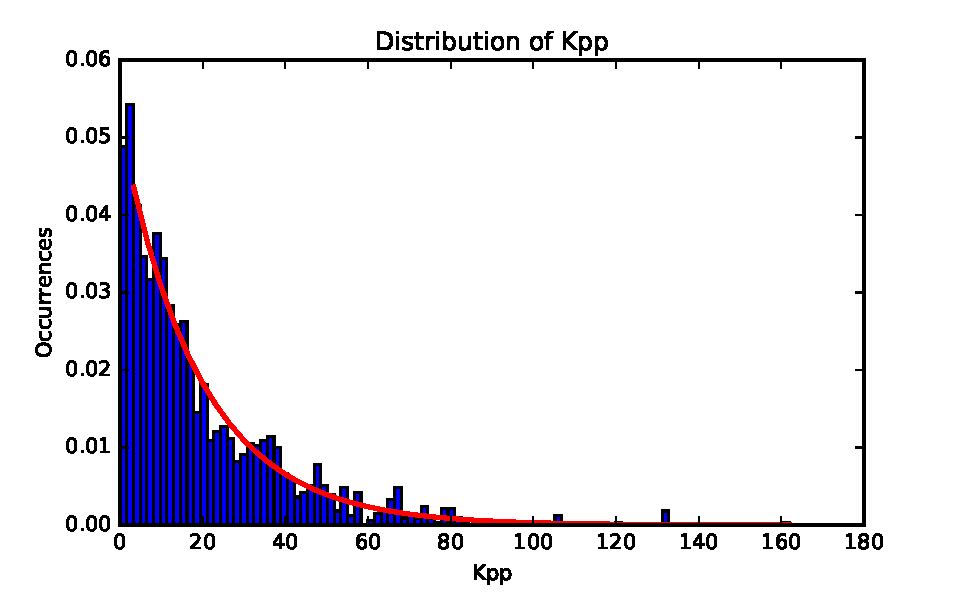
\includegraphics[width=8cm]{figures/kpp.pdf}
\caption{An example fitted parameter distribution. This example shows the sampled distribution of fitted parameter for expression reaction of \texttt{Pu.1}, \texttt{$k_1$}. }  \label{fig:04}
\end{figure}

\begin{table}[h]
\begin{center}
\begin{tabular}{|l | c | c | c |}
\hline
Parameter & Shape & Scale & Expected \\
\hline
\texttt{$k_1$} & 0.9910 & 19.5851 & 19.4089 \\
\texttt{$k_2$} & 1.0695 & 18.2771 & 19.4570 \\
\texttt{$k_3$} & 1.0366 & 0.4757 & 0.4931 \\
\texttt{$k_4$} & 1.0520 & 0.4837 & 0.5089 \\
\texttt{$K_{P1}$} & 1.0069 & 20.3016 & 20.4407 \\
\texttt{$K_{P2}$} & 0.9422 & 21.4545 & 20.2145 \\
\hline
\end{tabular}

\vspace*{5pt}

\caption{The fitted shapes and scales of the underlying parameter disribution for all parameters involved in linear decision process. The values were fitted from the distribution of parameters sampled from all simulated particles. An example of such distribution could be seen in Figure \ref{fig:04}). In that example, the red line was the probability density function of the gamma distribution underlying the parameter.}
\end{center}
\label{tab:01}
\end{table}

\vspace*{-12pt}

\section{Discussion}

The model is based on the theory that a cross inhibition of the transcription factors \texttt{$K_{P1}$} and \texttt{$K_{P2}$} results in a switch like behavior of the transcription factors, which in turn governs the CMP lineage decision. Our results however cannot support this hypothesis as the fitted model parameters \texttt{{$K_{P1}$}} and \texttt{{$K_{P2}$}}, which represent the concentrations at which the production inhibition of \texttt{Gata1} and \texttt{Pu.1} through the transcription factors is at half its maximum value, are significantly higher than the actual concentrations of \texttt{Pu.1} and \texttt{Gata.1} present in the time series data. This suggests that almost no inhibitory effect is apparent in the experiment. Furthermore the high similarity between both the production and degradation ratios of the transcription factors cannot account for uneven outcome of lineage decision via stochastic process.

\vspace*{-12pt}

\section{Conclusion}

In the course of this project we managed to implement the Particle Filter Algorithm as a framework for the inference of model parameters through the use of time series data. The resulting fitted parameters did not support our initial hypothesis of a cross inhibition between \textit{Gata1} and \textit{Pu.1}. This finding was also confirmed by other publication which used the same data set claiming independence of early myeloid lineage choice with regards to the transcription factors \texttt{Pu.1} and \texttt{Gata.1} (\citealp{Hoppe16}). This highlights our framework's capability to convey underlying mechanics prior unknown to us. We also show that our framework can be used to compare model performance with regards to experimental data. This in turn hallmarks our framework potential as supporting tool for research scientists.

\vspace*{-6pt}

%\begin{figure}[!tpb]%figure1
%\fboxsep=0pt\colorbox{gray}{\begin{minipage}[t]{235pt} \vbox to 100pt{\vfill\hbox to
%235pt{\hfill\fontsize{24pt}{24pt}\selectfont FPO\hfill}\vfill}
%\end{minipage}}
%%\centerline{\includegraphics{fig01.eps}}
%\caption{Caption, caption.}\label{fig:01}
%\end{figure}

%\begin{figure}[!tpb]%figure2
%%\centerline{\includegraphics{fig02.eps}}
%\caption{Caption, caption.}\label{fig:02}
%\end{figure}


\section*{Acknowledgements}

We would like to express our gratitude to Werner Mewes, Fabian Theis, Jan Quell and Anna Dieckman for facilitating the project. We would also like to thanks Philipp S. Hoppe, Michael Schwarzfischer, Dirk Loeffler, Konstantinos D. Kokkaliaris, Oliver Hilsenbeck, Nadine Moritz, Max Endele, Adam Filipczyk, Adriana Gambardella, Nouraiz Ahmed, Martin Etzrodt, Daniel L. Coutu, Michael A. Rieger, Bernhard Schauberger, Ingo Burtscher, Olga Ermakova, Antje B\"urger, Heiko Lickert, Claus Nerlov and Timm Schroder who agreed to provide us with the experiment data, without which we wouldn't be able to test our framework and models.

\vspace*{-18pt}

\section*{Funding}

We acknowledge the fact that the project and corresponding projects this project is based on are, directly and undirectly, financed by several grants given to following institutes within the Helmholtz Zentrum M\"unchen: the Institute of Bioinformatics and Systems Biology, the Institute of Computational Biology, the Institute of Diabetes and Regeneration Research, the Institute of Development Genetics and the Research Unit Stem Cell Dynamics. Some grants might also be involved coming from following institutions: Department of Biosystems Science and Engineering at ETH Zurich, MRC Molecular Haematology Unit at University of Oxford, Institute di Biologia Cellulare e Neurobiologia at CNR, Beta Cell Biology at the Medical Faculty of the Technical University of Munich, Department of Mathematics at the Technical University of Munich and EMBL Mouse Biology Unit.\vspace*{-12pt}

%\bibliographystyle{natbib}
%\bibliographystyle{achemnat}
%\bibliographystyle{plainnat}
%\bibliographystyle{abbrv}
%\bibliographystyle{bioinformatics}
%
%\bibliographystyle{plain}
%
%\bibliography{Document}

\vspace*{15pt}

\begin{thebibliography}{}

\bibitem[Feigelman, 2016]{Feigelman16}
Feigelman, J. (2016). "Stochastic and deterministic methods for the analysis of Nanog dynamics in mouse embryonic stem cells." PhD Thesis, Technische Universit\"at M\"unchen, Munich, Germany.\vspace*{-2pt}

\bibitem[Hoppe {\it et~al}, 2016]{Hoppe16}
Hoppe, P.S., Schwarzfischer, M., Loeffler, D.,  Kokkaliaris, K.D., Hilsenbeck, O., Mortz, N., ... \& Etzrodt, M. (2016). Early myeloid lineage choice is not initiated by random PU.1 to GATA1 protein ratios. \textit{Nature}, \textbf{535(7611)}, 299-302.

\bibitem[Graf \& Enver, 2009]{Graf09}
Graf, T., \& Enver, T. (2009). Forcing cells to change lineages. \textit{Nature}, \textbf{462(7273)}, 587-594.

\bibitem[Elowitz {\it et~al}, 2016]{Elowitz02}
Elowitz, M. B., Levine, A. J., Siggia, E. D., \& Swain, P. S. (2002). Stochastic gene expression in a single cell. \textit{Science}, \textbf{297(5584)}, 1183-1186.

\bibitem[Orkin {\it et~al}, 2008]{Orkin08}
Orkin, S. H., \& Zon, L. I. (2008). Hematopoiesis: an evolving paradigm for stem cell biology. \textit{Cell}, \textbf{132(4)}, 631-644.

\bibitem[Filipczyk {\it et~al}, 2015]{Filipczyk15}
Filipczyk, A., Marr, C., Hastreiter, S., Feigelman, J., Schwarzfischer, M., Hoppe, P. S., ... \& Hilsenbeck, O. (2015). Network plasticity of pluripotency transcription factors in embryonic stem cells. \textit{Nature cell biology}.

\bibitem[Doucet {\it et~al}, 1945]{Doucet01}
Doucet, A., De Freitas, N., \& Gordon, N. (2001). An introduction to sequential Monte Carlo methods. In \textit{Sequential Monte Carlo methods in practice} (pp. 3-14). Springer New York.

\bibitem[Liu and Chen, 1998]{Liu98}
Liu, J. S., \& Chen, R. (1998). Sequential Monte Carlo methods for dynamic systems. \textit{Journal of the American statistical association}, 93(443), 1032-1044.

\bibitem[Del Moral, 1996]{DelMoral96}
Del Moral, P. (1996). Non-linear filtering: interacting particle resolution. \textit{Markov processes and related fields}, \textbf{2(4)}, 555-581.

\bibitem[Del Moral, 2012]{DelMoral12}
Del Moral, P., Doucet, A., \& Jasra, A. (2012). On adaptive resampling strategies for sequential Monte Carlo methods. \textit{Bernoulli}, \textbf{18(1)}, 252-278.

\bibitem[Gillespie, 1977]{Gillespie77}
Gillespie, D. T. (1977). Exact stochastic simulation of coupled chemical reactions. \textit{The journal of physical chemistry}, \textbf{81(25)}, 2340-2361.

\bibitem[Doob, 1945]{Doob45}
Doob, J. L. (1945). Markoff chains--denumerable case. \textit{Transactions of the American Mathematical Society}, \textbf{58(3)}, 455-473.

\bibitem[Chung, 1967]{Chung67}
Chung, K. L. (1967). \textit{Markov Chain}. Berlin: Springer-Verlag.

\bibitem[Gillespie, 2007]{Gillespie07}
Gillespie, D. T. (2007). Stochastic simulation of chemical kinetics. \textit{Annu. Rev. Phys. Chem.}, \textbf{58}, 35-55.

\bibitem[Fahrmeir {\it et~al}., 2007]{Fahrmeir07}
Fahrmeir, L., K\"unstler, R., Pigeot, I., \& Tutz, G. (2007). \textit{Statistik: Der Weg zur Datenanalyse}. Springer-Verlag.

\bibitem[Wilkinson, 2011]{Wilkinson11}
Wilkinson, D. J. (2011). Stochastic modelling for systems biology. CRC press.

\bibitem[Zechner {\it et~al}., 2011]{Zechner11}
Zechner, C., Pelet, S., Peter, M., \& Koeppl, H. (2011, December). Recursive Bayesian estimation of stochastic rate constants from heterogeneous cell populations. In \textit{2011 50th IEEE Conference on Decision and Control and European Control Conference} (pp. 5837-5843). IEEE.

\bibitem[Haseltine {\it et~al}., 2005]{Haseltine05}
Haseltine, E. L., \& Rawlings, J. B. (2005). On the origins of approximations for stochastic chemical kinetics. \textit{The Journal of chemical physics}, \textbf{123(16)}, 164115.

\bibitem[Sherlock {\it et~al}., 2014]{Sherlock14}
Sherlock, C., Golightly, A., \& Gillespie, C. S. (2014). Bayesian inference for hybrid discrete-continuous stochastic kinetic models. \textit{Inverse Problems}, \textbf{30(11)}, 114005.

\bibitem[Posada and Buckley, 2014]{PosadaBuckley14}
Posada, D., \& Buckley, T. R. (2004). Model selection and model averaging in phylogenetics: advantages of Akaike information criterion and Bayesian approaches over likelihood ratio tests. \textit{Systematic biology}, \textbf{53(5)}, 793-808.

\bibitem[Bozdogan, 1987]{Bozdogan87}
Bozdogan, H. (1987). Model selection and Akaike's information criterion (AIC): The general theory and its analytical extensions. \textit{Psychometrika}, \textbf{52(3)}, 345-370.

\bibitem[Wilkinson, 2010]{Wilkinson10}
Wilkinson, D. J. (2010). Parameter inference for stochastic kinetic models of bacterial gene regulation: a Bayesian approach to systems biology. In \textit{Proceedings of 9th Valencia International Meeting on Bayesian Statistics}. Oxford University Press (pp. 679-705).

\bibitem[Golightly and Wilkinson, 2010]{GolightlyWilkinson10}
Golightly, A., \& Wilkinson, D. J. (2010). Markov chain Monte Carlo algorithms for SDE parameter estimation. \textit{Learning and Inference for Computational Systems Biology}, 253-276.

\bibitem[Gonzales {\it et~al}., 2013]{Gonzales13}
Gonzalez, A., Uhlendorf, J., Schaul, J., Cinquemani, E., Batt, G., \& Ferrari-Trecate, G. (2013). \textit{Identification of biological models from single-cell data: a comparison between mixed-effects and moment-based inference} (Doctoral dissertation, INRIA).

\bibitem[Komorowski {\it et~al}., 2009]{Komorowski09}
Komorowski, M., Finkenstädt, B., Harper, C. V., \& Rand, D. A. (2009). Bayesian inference of biochemical kinetic parameters using the linear noise approximation. \textit{BMC bioinformatics}, \textbf{10(1)}, 1.

\end{thebibliography}
\end{document}
